The statistical evaluation of the random number generators discussed here employs a selection of tests primarily based on the NIST SP 800-22 standard. The specific software implementation of these statistical tests utilized for this research is adapted from the open-source Python suite developed by Steven Kho Ang, an IT Professional. This foundational codebase is publicly available for reference on GitHub: \url{https://github.com/stevenang/randomness_testsuite}. The subsequent sections detail the outcomes and interpretations of these tests as applied to the evaluated random number generation methods.

\begin{table*}[htbp]
\centering
\caption{Summary of NIST SP 800-22 Rev 1a Test Results for Various RNGs ($\alpha = 0.01$)}
\label{tab:nist_results_all_five_rngs}
\resizebox{\textwidth}{!}{%
\begin{tabular}{|l|cc|cc|cc|cc|cc|}
\hline
\textbf{NIST Test} & \multicolumn{2}{c|}{\textbf{CRNG}} & \multicolumn{2}{c|}{\textbf{CTR DRBG (no seq)} } & \multicolumn{2}{c|}{\textbf{CTR DRBG (seq)}} & \multicolumn{2}{c|}{\textbf{BEACON}} & \multicolumn{2}{c|}{\textbf{QRNG}} \\
& \textbf{P-value} & \textbf{Result} & \textbf{P-value} & \textbf{Result} & \textbf{P-value} & \textbf{Result} & \textbf{P-value} & \textbf{Result} & \textbf{P-value} & \textbf{Result} \\
\hline
Frequency (Monobit) & $0.779467$ & Pass & $0.671566$ & Pass & $0.499041$ & Pass & $0.852445$ & Pass & $0.000000$ & Fail \\
Frequency within a Block (M=128) & $0.133136$ & Pass & $0.774426$ & Pass & $0.600071$ & Pass & $0.627412$ & Pass & $0.888434$ & Pass \\
Runs Test & $0.362484$ & Pass & $0.821062$ & Pass & $0.490481$ & Pass & $0.723313$ & Pass & $0.000000$ & Fail \\
Maurer's Universal (L=see note) & $0.904546$ (L=6) & Pass & $0.212853$ (L=7) & Pass & $0.098342$ (L=7) & Pass & $0.799200$ (L=7) & Pass & $0.547755$ (L=6) & Pass \\
Cumulative Sums (Forward) & $0.725570$ & Pass & $0.632885$ & Pass & $0.708291$ & Pass & $0.433978$ & Pass & $0.000000$ & Fail \\
Cumulative Sums (Backward) & $0.950381$ & Pass & $0.970669$ & Pass & $0.665229$ & Pass & $0.585944$ & Pass & $0.000000$ & Fail \\
\hline
\end{tabular}%
}
\begin{flushleft}
\footnotesize Note: "Result" indicates Pass (P-value $\ge 0.01$) or Fail (P-value $< 0.01$). M and L values for specific tests are based on implementation defaults or sequence length (M=128 for Block Frequency). For Maurer's Universal Test, L was determined by sequence length: L=6 for n=500,000 (CRNG, QRNG); L=7 for n=1,000,000 (CTR DRBG (no seq),CTR DRBG (seq), BEACON). CRNG and QRNG tested on 500,000-bit sequences. CTR DRBG (no seq), CTR DRBG (seq) and BEACON tests performed on a 1,000,000-bit segment
\end{flushleft}
\end{table*}

For comparative analysis, the following results of different generators will be compared with a classical pseudo-random bit (CRNG) strings. These sequences were produced using Python's standard \texttt{random} module, where each bit was independently determined by the \texttt{random.choice(['0', '1'])} function to form strings of the required length.


\subsection{\textbf{Histogram}}


\begin{figure}[htbp] 
    \centering 
    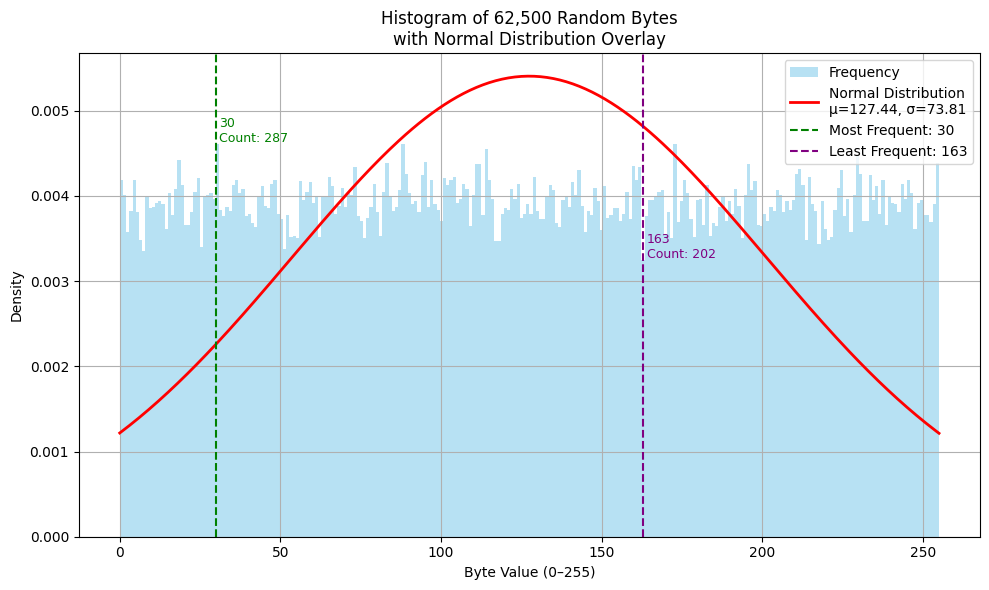
\includegraphics[width=0.9\columnwidth]{images/Hist_CRNG.png} 
    \caption{Histogram: CRNG}
    \label{fig:H:CRNG}
\end{figure}

The histogram corresponding to 62{,}500 random bytes generated by the Classical Random Number Generator (CRNG) exhibits a distribution that appears reasonably uniform, indicating a satisfactory degree of randomness. The sample mean ($\mu = 127.44$) and standard deviation ($\sigma = 73.81$) are closely aligned with the theoretical values for a perfectly uniform distribution of bytes in the range 0--255, namely $\mu_{\text{th}} = 127.5$ and $\sigma_{\text{th}} \approx 73.90$.

The most frequently occurring byte appears 287 times, while the least frequent appears 202 times. These values are centered around the expected average count of approximately $244.14$ (computed as $62500 / 256$). Taken together, these statistical properties support the conclusion that the CRNG produces high-quality random byte sequences.


\subsection{Statistical Test Results for the CTR DRBG Implementation} 

The output sequence from the Counter Mode Deterministic Random Bit Generator (CTR DRBG was evaluated. While a total of 50,000,000 bits were generated, the statistical tests detailed herein were performed on a 1,000,000-bit segment, confirmed to be purely binary.

\subsubsection{\textbf{Frequency (Monobit) Test}}
This test assesses the overall balance of zeros and ones. The CTR DRBG yielded a P-value of $0.671566$, resulting in a 'Pass' conclusion. This indicates that the overall proportion of zeros and ones in the tested sequence is statistically balanced and consistent with random data.

\subsubsection{\textbf{Frequency Test within a Block}}
This test examines the proportion of ones within M-bit blocks for local uniformity. The CTR DRBG sequence produced a P-value of $0.774426$, leading to a 'Pass' status. This suggests that the distribution of ones and zeros is statistically uniform when examined across smaller, localized blocks (using M=\texttt{128}, the default from the implementation if not otherwise specified for this run).

\subsubsection{\textbf{Runs Test}}
The Runs Test evaluates the rate of oscillation between zeros and ones. The CTR DRBG achieved a P-value of $0.821062$, corresponding to a 'Pass'. This implies that the number of runs of zeros and ones is as expected for a random sequence, indicating healthy oscillation patterns.

\subsubsection{\textbf{Maurer's "Universal Statistical" Test}}
This test assesses the sequence's compressibility. The CTR DRBG data resulted in a P-value of $0.212853$, and a 'Pass' conclusion. This indicates that, according to this test, the sequence does not exhibit significant compressibility, a characteristic consistent with random data (using L=\texttt{12}, as determined by the implementation for a 50,000,000-bit sequence).

\subsubsection{\textbf{Cumulative Sums (Cusum) Test}}
This test checks for maximal excursions in a random walk derived from the sequence. For the forward test, the CTR DRBG yielded a P-value of $0.632885$, resulting in a 'Pass'. Similarly, for the backward test, the P-value was $0.970669$, also a 'Pass'. Collectively, these 'Pass' results suggest that the cumulative sum of the sequence does not drift excessively from zero in either direction, indicating no significant overall bias or trends in the data.

\subsubsection{\textbf{Histogram}}


\begin{figure}[htbp] 
    \centering 
    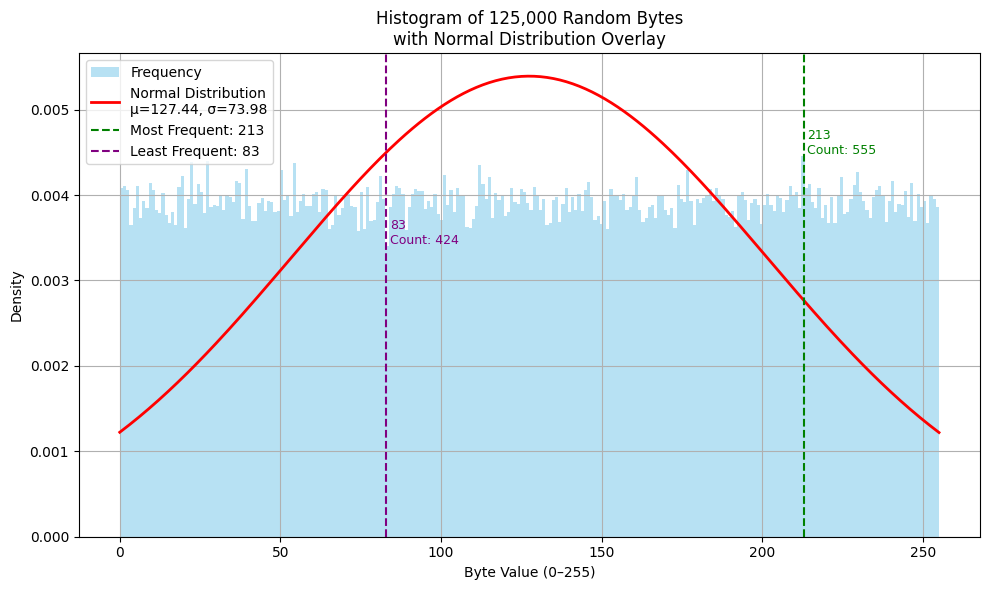
\includegraphics[width=0.9\columnwidth]{images/Hist_CTR.png} 
    \caption{Histogram: CTR-DRBG}
    \label{fig:H:CTR}
\end{figure}

This histogram represents 125,000 random bytes from the CTR generator. The visual distribution of byte frequencies appears largely uniform, which is indicative of a high degree of randomness. The sample mean extracted from the data is $\mu = 127.44$, and the sample standard deviation is $\sigma = 73.98$. These values align closely with the theoretical figures for a perfect uniform distribution over the 0-255 byte range ($\mu_{th} = 127.5$ and $\sigma_{th} \approx 73.90$). The most frequent byte value was observed 555 times, and the least frequent was observed 424 times. For this sample size, the expected average count per byte is approximately $488.28$ ($125000 / 256$). The proximity of the observed mean and standard deviation to the theoretical values, along with the reasonable concentration of extreme counts around the expected average, supports the conclusion that the CTR generator produces random bytes of good quality.

\noindent 
In summary, the statistical evaluation of this 1,000,000-bit sequence from the CTR DRBG implementation demonstrates excellent random characteristics across all five selected NIST tests. The sequence successfully passed tests for bit frequency (both global and local), run properties, compressibility, and cumulative sum trends, indicating a high degree of conformity with the expected properties of a random sequence at the chosen significance level.

\subsection{Statistical Test Results for the CTR DRBG (Sequential Seed) Implementation} 

The output sequence from the Counter Mode Deterministic Random Bit Generator with sequential seeding (CTR DRBG (seq)) was evaluated. While a total of 400,000,000 bits were generated, the statistical tests detailed herein were performed on a 1,000,000-bit segment, confirmed to be purely binary. 

\subsubsection{\textbf{Frequency (Monobit) Test}}
This test assesses the overall balance of zeros and ones. The CTR DRBG (seq) yielded a P-value of $0.671566$, resulting in a 'Pass' conclusion. This indicates that the overall proportion of zeros and ones in the tested 1,000,000-bit sequence is statistically balanced and consistent with random data.

\subsubsection{\textbf{Frequency Test within a Block}}
This test examines the proportion of ones within M-bit blocks for local uniformity. The CTR DRBG (seq) sequence produced a P-value of $0.600071$, leading to a 'Pass' status. This suggests that the distribution of ones and zeros is statistically uniform when examined across smaller, localized blocks (using M=\texttt{128}, the default from the implementation if not otherwise specified for this run).

\subsubsection{\textbf{Runs Test}}
The Runs Test evaluates the rate of oscillation between zeros and ones. The CTR DRBG (seq) achieved a P-value of $0.490481$, corresponding to a 'Pass'. This implies that the number of runs of zeros and ones is as expected for a random sequence, indicating healthy oscillation patterns.

\subsubsection{\textbf{Maurer's "Universal Statistical" Test}}
This test assesses the sequence's compressibility. The CTR DRBG (seq) data resulted in a P-value of $0.098342$, and a 'Pass' conclusion. This indicates that, according to this test, the 1,000,000-bit sequence does not exhibit significant compressibility, a characteristic consistent with random data (using L=\texttt{7}, as determined by the implementation for this sequence length).

\subsubsection{\textbf{Cumulative Sums (Cusum) Test}}
This test checks for maximal excursions in a random walk derived from the sequence. For the forward test, the CTR DRBG (seq) yielded a P-value of $0.708291$, resulting in a 'Pass'. Similarly, for the backward test, the P-value was $0.665229$, also a 'Pass'. Collectively, these 'Pass' results suggest that the cumulative sum of the sequence does not drift excessively from zero in either direction, indicating no significant overall bias or trends in the data.

\subsubsection{\textbf{Histogram}}


\begin{figure}[htbp] 
    \centering 
    \includegraphics[width=0.9\columnwidth]{images/Hist_seq.png} 
    \caption{Histogram: CTR-DRBG(seq)}
    \label{fig:H:CTR(seq)}
\end{figure}

This histogram represents 125,000 random bytes from the SEQ generator. The visual distribution of byte frequencies appears largely uniform, which is indicative of a high degree of randomness. The sample mean extracted from the data is $\mu = 127.29$, and the sample standard deviation is $\sigma = 73.94$. These values align closely with the theoretical figures for a perfect uniform distribution over the 0-255 byte range ($\mu_{th} = 127.5$ and $\sigma_{th} \approx 73.90$). The most frequent byte value was observed 541 times, and the least frequent was observed 413 times. For this sample size, the expected average count per byte is approximately $488.28$ ($125000 / 256$). The proximity of the observed mean and standard deviation to the theoretical values, along with the reasonable concentration of extreme counts around the expected average, supports the conclusion that the SEQ generator produces random bytes of good quality.

\noindent 

In summary, the statistical evaluation of the 1,000,000-bit segment from the CTR DRBG (seq) implementation demonstrates robust random characteristics across all five selected NIST tests. The sequence successfully passed tests for bit frequency (both global and local), run properties, compressibility, and cumulative sum trends, indicating a high degree of conformity with the expected properties of a random sequence at the chosen significance level.

\subsection{Statistical Test Results for the BEACON Generator} % Updated section title

The output sequence from the BEACON generator was evaluated using a 1,000,000-bit segment of entire sample of 8,681,984, confirmed to be purely binary. 

\subsubsection{\textbf{Frequency (Monobit) Test}}
This test assesses the overall balance of zeros and ones. The BEACON generator yielded a P-value of $0.852445$, resulting in a 'Pass' conclusion. This indicates that the overall proportion of zeros and ones in the tested sequence is statistically balanced.

\subsubsection{\textbf{Frequency Test within a Block}}
This test examines the proportion of ones within M-bit blocks for local uniformity. The BEACON sequence produced a P-value of $0.627412$, leading to a 'Pass' status. This suggests that the distribution of ones and zeros is statistically uniform when examined across smaller, localized blocks (using M=\texttt{128}, the default from the implementation).

\subsubsection{\textbf{Runs Test}}
The Runs Test evaluates the rate of oscillation between zeros and ones. The BEACON generator achieved a P-value of $0.723313$, corresponding to a 'Pass'. This implies that the number of runs of zeros and ones is as expected for a random sequence.

\subsubsection{\textbf{Maurer's "Universal Statistical" Test}}
This test assesses the sequence's compressibility. The BEACON data resulted in a P-value of $0.799200$, and a 'Pass' conclusion. This indicates that, according to this test, the sequence does not exhibit significant compressibility, a characteristic consistent with random data (using L=\texttt{7}, as determined by the implementation for a 1,000,000-bit sequence).

\subsubsection{\textbf{Cumulative Sums (Cusum) Test}}
This test checks for maximal excursions in a random walk derived from the sequence. For the forward test, the BEACON generator yielded a P-value of $0.433978$, resulting in a 'Pass'. Similarly, for the backward test, the P-value was $0.585944$, also a 'Pass'. Collectively, these 'Pass' results suggest that the cumulative sum of the sequence does not drift excessively from zero in either direction, indicating no significant overall bias or trends in the data according to this specific test.

\subsubsection{\textbf{Histogram}}


\begin{figure}[htbp] 
    \centering 
    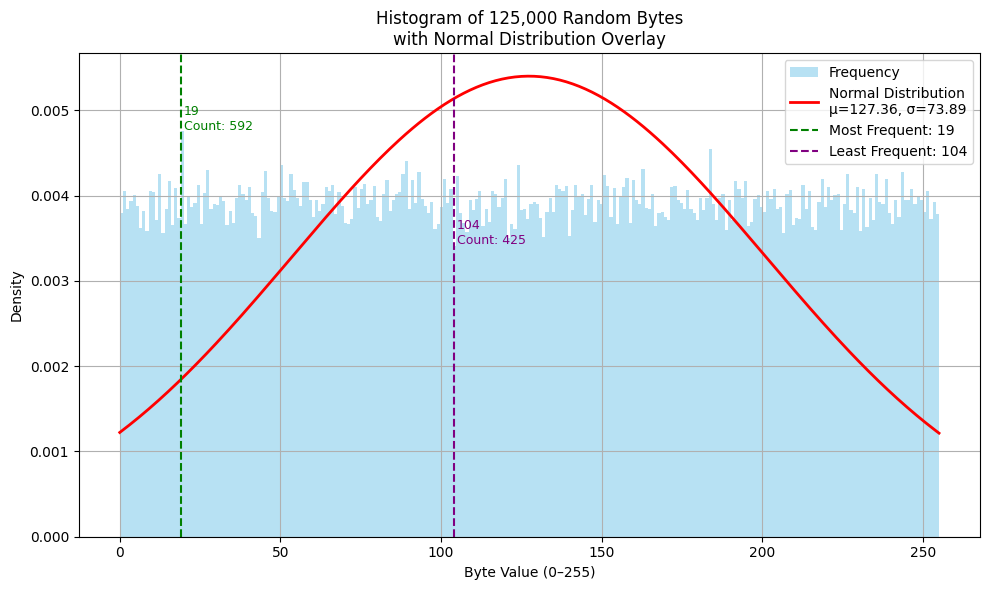
\includegraphics[width=0.9\columnwidth]{images/HIST_Beacon.png} 
    \caption{Histogram: BEACON}
    \label{fig:H:BEACON}
\end{figure}

This histogram represents 125,000 random bytes from the Beacon generator. The visual distribution of byte frequencies appears largely uniform, which is indicative of a high degree of randomness. The sample mean extracted from the data is $\mu = 127.36$, and the sample standard deviation is $\sigma = 73.89$. These values align closely with the theoretical figures for a perfect uniform distribution over the 0-255 byte range ($\mu_{th} = 127.5$ and $\sigma_{th} \approx 73.90$). The most frequent byte value was observed 592 times, and the least frequent was observed 425 times. For this sample size, the expected average count per byte is approximately $488.28$ ($125000 / 256$). The proximity of the observed mean and standard deviation to the theoretical values, along with the reasonable concentration of extreme counts around the expected average, supports the conclusion that the Beacon generator produces random bytes of good quality.

\noindent 

Based on these five selected NIST tests, the 1,000,000-bit segment from the BEACON generator passed tests for bit frequency (global and local), run properties, compressibility, and cumulative sum trends. Therefore the BEACON generator exhibits random characteristics.

\subsubsection{Statistical Test Results for the Quantum RNG (QRNG)}

The output sequence from the quantum random number generator (QRNG), consisting of 500,000 bits confirmed to be purely binary, was evaluated using five selected statistical tests from the NIST SP 800-22 Rev 1a suite.

\subsubsection{\textbf{Frequency (Monobit) Test}}
This test assesses the overall balance of zeros and ones. The QRNG yielded a P-value of $0.000000$, resulting in a 'Fail' conclusion. This indicates a critical imbalance in the global proportion of zeros and ones within the tested sequence.

\subsubsection{\textbf{Frequency Test within a Block}}
This test examines the proportion of ones within M-bit blocks for local uniformity. The QRNG sequence produced a P-value of $0.888434$, leading to a 'Pass' status. This suggests that while a global imbalance exists, the distribution of ones and zeros appears statistically uniform when analyzed across smaller, localized blocks (e.g., using M=\texttt{128}).

\subsubsection{\textbf{Runs Test}}
The Runs Test evaluates the rate of oscillation between zeros and ones. The QRNG achieved a P-value of $0.000000$, corresponding to a 'Fail'. This implies that the total number of runs of zeros and ones deviates significantly from what is expected for a random sequence, indicating problematic oscillation patterns.

\subsubsection{\textbf{Maurer's "Universal Statistical" Test}}
This test assesses the sequence's compressibility. The QRNG data resulted in a P-value of $0.547755$, and a 'Pass' conclusion. This indicates that, according to this test, the sequence does not exhibit significant compressibility, a characteristic consistent with random data (using L=\texttt{6}, as determined by the implementation for a 500,000-bit sequence).

\subsubsection{\textbf{Cumulative Sums (Cusum) Test}}
This test checks for maximal excursions in a random walk derived from the sequence. For the forward test, the QRNG yielded a P-value of $0.000000$, resulting in a 'Fail'. Similarly, for the backward test, the P-value was $0.000000$, also a 'Fail'. These 'Fail' results across both modes strongly suggest that the cumulative sum of the sequence deviates excessively from zero, pointing to substantial trends or biases within the data.

\subsubsection{\textbf{Histogram}}


\begin{figure}[htbp] 
    \centering 
    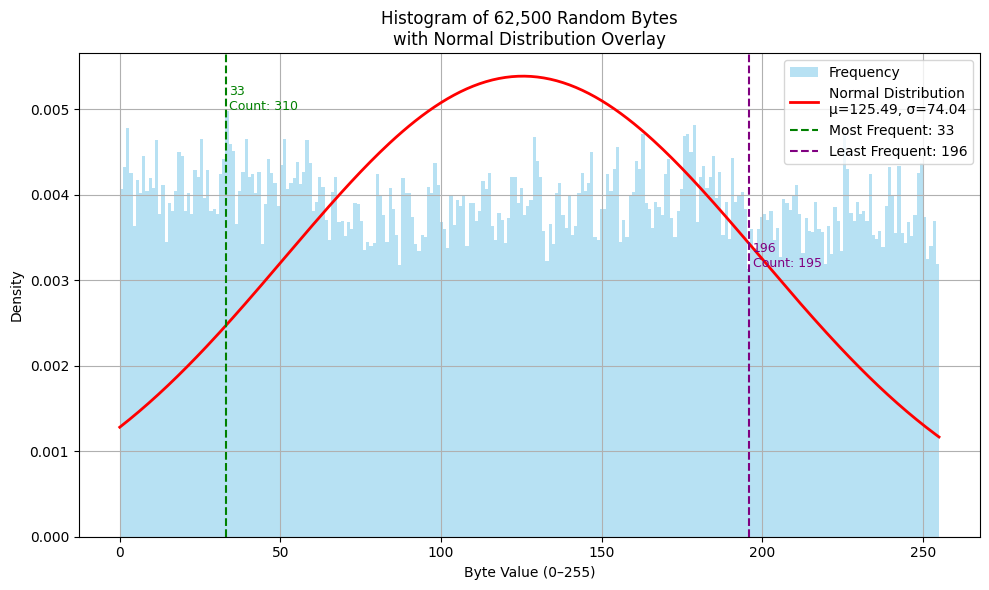
\includegraphics[width=0.9\columnwidth]{images/Hist_QRNG.png} 
    \caption{Histogram: QRNG}
    \label{fig:H:QRNG}
\end{figure}

The histogram displays data for 62,500 random bytes from the QRNG (Quantum Random Number Generator). The distribution of byte frequencies approximates uniformity, indicating some degree of randomness. The sample mean is $\mu = 125.49$, which is slightly lower than the theoretical mean of $127.5$ for an ideal uniform distribution. The sample standard deviation is $\sigma = 74.04$, closely matching the theoretical standard deviation of $\approx 73.90$. The most frequent byte occurred 310 times, while the least frequent byte occurred 195 times. The expected average count per byte value for this sample size is approximately $244.14$ ($62500 / 256$). While the standard deviation is good, the slight deviation in the mean and the spread of frequency counts (from 195 to 310) suggest that while generally random, the output might benefit from further statistical tests to confirm ideal uniformity.

\noindent 

In summary, the evaluation of this 500,000-bit sequence from the QRNG reveals significant statistical weaknesses. Despite passing tests for local frequency distribution (Block Frequency) and compressibility (Maurer's Universal), the QRNG critically fails the fundamental Frequency (Monobit) test, the Runs Test, and both Cumulative Sums tests. These failures point to considerable issues with overall bit bias, the nature of bit alternations, and pervasive trends within the generated sequence, suggesting notable deviations from ideal randomness.
